\documentclass{book}

% Configuration
% ------------------
% Packages
% ------------------
\usepackage[english]{babel}
\usepackage[T1]{fontenc}
\usepackage[scaled]{helvet}
\usepackage[utf8]{inputenc}
\usepackage[letterpaper]{geometry}
\usepackage[dvipsnames]{xcolor}

\usepackage{algorithmicx}
\usepackage{amsfonts,amsmath,amsthm,amssymb}
\usepackage{booktabs}
\usepackage{dsfont}
\usepackage{float}
\usepackage{graphicx}
\usepackage{latexsym}
\usepackage{mathtools}
\usepackage{sectsty}
\usepackage{setspace}
\usepackage{subcaption}
\usepackage{tabularx}
\usepackage{tikz}
\usepackage{tikz-3dplot}
% \usepackage{txfonts}
\usepackage{url}
\usepackage{wrapfig}
\usepackage{xparse}

% ------------------
% Shortcuts
% ------------------
\newcommand{\N}{\mathbb{N}}
\newcommand{\R}{\mathbb{R}}
\newcommand{\C}{\mathbb{C}}
\newcommand{\Z}{\mathbb{Z}}

\newcommand{\complexspace}[1]{\complexset^{#1}}
\newcommand{\realspace}[1]{\realset^{#1}}

\newcommand{\inverse}[1]{{#1}^{-1}}
\newcommand{\transpose}[1]{{#1}^{\top}}

\newcommand{\vdim}[1]{\mathrm{dim}\left( #1 \right)}
\newcommand{\vrank}[1]{\mathrm{rk}\left( #1 \right)}
\newcommand{\vspan}[1]{\mathrm{span}\left[ #1 \right]}

\newcommand{\id}{\mathrm{id}}
\newcommand{\GL}{\mathrm{GL}}
\newcommand{\sgn}{\mathrm{sgn}}

\newcommand{\im}[1]{\mathrm{Im}\left( #1 \right)}

\def\lcirclearrowleft{\ensuremath{%
  \rotatebox[origin=c]{180}{$\circlearrowleft$}}}
\def\lcirclearrowright{\ensuremath{%
  \rotatebox[origin=c]{180}{$\circlearrowright$}}}

\newcommand{\actson}{~\lcirclearrowright~}

% ------------------
% Command Redefinitions
% ------------------
\renewcommand{\qed}{\hfill$\blacksquare$}

\makeatletter
\renewcommand*\env@matrix[1][*\c@MaxMatrixCols c]{%
    \hskip -\arraycolsep
    \let\@ifnextchar\new@ifnextchar
    \array{#1}}
\makeatother

\renewcommand{\phi}{\varphi}
\renewcommand{\ker}[1]{\mathrm{ker}\left( #1 \right)}

% ------------------
% Colors
% ------------------
\definecolor{primary}{HTML}{207BA5}
\definecolor{greybg}{RGB}{249, 249, 249}

\definecolor{thmbg}{HTML}{F2F2F9}
\definecolor{lemmabg}{HTML}{FFFAF8}
\definecolor{lemmafr}{HTML}{983b0f}
\definecolor{propbg}{HTML}{f2fbfc}
\definecolor{propfr}{HTML}{191971}
\definecolor{myp}{RGB}{197, 92, 212}
\definecolor{grey17}{RGB}{17, 17, 17}
\definecolor{MyGrey}{HTML}{5B5B5B}

\definecolor{lightBlue}{rgb}{0.0, 0.64, 1.0}
\definecolor{lightRed}{rgb}{1.0, 0.50, 0.50}
\definecolor{darkGreen}{rgb}{0.31, 0.54, 0.30}
\definecolor{violet}{RGB}{186, 153, 242}

%----------------
%	Text Styles
%----------------
\DeclareTextFontCommand{\term}{\color{orange}\bfseries}
\DeclareTextFontCommand{\bred}{\color{red}\bfseries}
\DeclareTextFontCommand{\itblue}{\color{lightBlue}\itshape}

\DeclareTextFontCommand{\vector}{\bfseries\itshape}

% ------------------
%   URL Color
% ------------------
\usepackage[colorlinks=true]{hyperref}
\hypersetup{
    colorlinks=true,
    linkcolor=black,
    filecolor=magenta,
    urlcolor=blue,
}

% ------------------
% Tikz Externalize
% ------------------
\usetikzlibrary{external}
\tikzexternalize[prefix=tikz/]
\tikzset{external/only named=true}

% ------------------
% Boxes
% ------------------
\usepackage[most]{tcolorbox}

\newcommand\fancybox[3]{%
    \tcbset{
        mybox/.style={
                enhanced,
                boxsep=0mm,
                opacityfill=0,
                overlay={
                        \coordinate (X) at ([xshift=-1mm, yshift=-1.5mm]frame.north west);
                        \node[align=right, text=#1, text width=2.5cm, anchor=north east] at (X) {\bf#2};
                        \draw[line width=0.5mm, color=#1] (frame.north west) -- (frame.south west);
                    }
            }
    }
    \begin{tcolorbox}[mybox]
        #3
    \end{tcolorbox}
}

\tcbuselibrary{theorems,skins,hooks}
\NewDocumentCommand\thmbox{m O{\Large #1} O{greybg} O{primary} O{number within=section}}
{
    \newtcbtheorem[#5]{#1}{\large #2}
    {%
        enhanced,
        breakable,
        colback = #3,
        frame hidden,
        boxrule = 0sp,
        borderline west = {2pt}{0pt}{#4},
        sharp corners,
        detach title,
        before upper = \tcbtitle\par\smallskip,
        coltitle = #4,
        fonttitle = \bfseries,
        description font = \mdseries,
        separator sign none,
        segmentation style={solid, #4}
    }
    {th}
}

\thmbox{Corollary}[Corollary][myp!10][myp!85!black]
\thmbox{Lemma}[Lemma][lemmabg][lemmafr]
\thmbox{Propo}[Proposition][propbg][propfr]
\thmbox{Defi}[Definition][primary!12][primary]
\thmbox{Notation}[Notation][white][grey17][no counter]
\thmbox{Theorem}[Theorem][primary!12][primary]
\thmbox{Remark}[Remark][grey17!10][grey17][no counter]

% ------------------
% Environments
% ------------------
\newenvironment{corollary}[1][]   {\begin{Corollary}{#1}{}}                               {\end{Corollary}}
\newenvironment{definition}[1][]  {\begin{Defi}{#1}{}}                                    {\end{Defi}}
\newenvironment{lemma}[1][]       {\begin{Lemma}{#1}{}}                                   {\end{Lemma}}
\newenvironment{proposition}[1][] {\begin{Propo}{#1}{}}                                   {\end{Propo}}
\newenvironment{remark}[1][]      {\begin{Remark}{#1}{}}                                  {\end{Remark}}
\newenvironment{theorem}[1][]     {\begin{Theorem}{#1}{}}                                 {\end{Theorem}}

\newenvironment{rtheorem}[2][]    {\begin{Theorem}{#1}{#2}}                               {\end{Theorem}}

\theoremstyle{definition}
\newtheorem*{exam}{\color{primary}Example}
% \newcommand{\example}[1]{\begin{exam}#1\end{exam}}
% \newenvironment{example}          {\begin{exam}} {\begin{flushright}${\color{primary}\diamondsuit}$\end{flushright} \end{exam}}
\newenvironment{example}          {\begin{exam}} {\hfill${\color{primary}\diamondsuit}$\end{exam}}

\theoremstyle{definition}
\newtheorem*{clm}{\color{MyGrey}Claim}
\newenvironment{claim}            {\begin{clm}} {\end{clm}}

% ------------------
% Lists
% ------------------
\usepackage{enumitem}

\newcommand{\cnumero}[2]{
    \tikz[baseline=(myanchor.base)]
    \node[minimum size=0.2cm,circle,
        inner sep=1pt,draw, #2,thick,fill=#2](myanchor)
    {\color{white}\bfseries\fontsize{8}{8}#1};}

\newcommand*{\itembolasazules}[1]{\protect\cnumero{#1}{primary}}

\newenvironment{listo} {\begin{enumerate}[label=\itembolasazules{\arabic*}]} {\end{enumerate}}
\newenvironment{listu} {\begin{itemize}  [label=$\color{primary} \bullet$]}  {\end{itemize}}

% ------------------
% Table of Contents
% ------------------
\usepackage{blindtext}
\usepackage{framed}
\usepackage{titletoc}
\usepackage{etoolbox}

\patchcmd{\tableofcontents}{\contentsname}{\contentsname}{}{}

\renewenvironment{leftbar}
{\def\FrameCommand{\hspace{6em}%
        {\color{primary}\vrule width 2pt depth 6pt}\hspace{1em}}%
    \MakeFramed{\parshape 1 0cm \dimexpr\textwidth-6em\relax\FrameRestore}\vskip2pt%
}
{\endMakeFramed}

\titlecontents{chapter}[0em]
{\vspace*{2\baselineskip}}
{\parbox{4.5em}{%
        \hfill\Huge\bfseries\color{primary}\thecontentslabel}%
    \vspace*{-2.3\baselineskip}\leftbar\textbf{\color{primary}\small\chaptername~\thecontentslabel}\\
}{}{\endleftbar}

\titlecontents{section}[8.4em]
{\contentslabel{3em}}{}{}
{\hspace{0.5em}\nobreak\itshape\color{primary}\contentspage}

\titlecontents{subsection}[11.4em]
{\contentslabel{3em}}{}{}
{\hspace{0.5em}\nobreak\itshape\color{primary}\contentspage}

% ------------------
% Chapters
% ------------------
\newtcolorbox{titlecolorbox}[1]{ %the box around chapter
    coltext=white,
    colframe=primary,
    colback=primary,
    boxrule=0pt,
    arc=0pt,
    notitle,
    width=4.8em,
    height=2.4ex,
    before=\hfill
}

\usepackage[explicit]{titlesec}

\makeatletter
\let\old@rule\@rule
\def\@rule[#1]#2#3{\textcolor{primary}{\old@rule[#1]{#2}{#3}}}
\makeatother

\titleformat{\chapter}[display]
{\Huge}
{}
{0pt}
{\begin{titlecolorbox}{}
        {\large\MakeUppercase{\bf\chaptername}}
    \end{titlecolorbox}
    \vspace*{-3.19ex}\noindent\rule{\textwidth}{0.4pt}
    \parbox[b]{\dimexpr\textwidth-4.8em\relax}{\raggedright\MakeUppercase{#1}}{\hfill\fontsize{70}{60}\selectfont{\color{primary}\thechapter}}
}
[]

\titleformat{name=\chapter,numberless}[display]
{\Huge}
{}
{0pt}
{
    \vspace*{-3.19ex}\noindent\rule{\textwidth}{0.4pt}
    \parbox[b]{\dimexpr\textwidth-4.8em\relax}{\raggedright\MakeUppercase{#1}}
}
[]

% ------------------
% Sections
% ------------------
\titleformat{\section}[hang]{\Large\bfseries}%
{\rlap{\color{primary}\rule[-6pt]{\textwidth}{0.4pt}}\colorbox{primary}{%
        \raisebox{0pt}[13pt][3pt]{ \makebox[60pt]{% height, width
                \selectfont\color{white}{\thesection}}
        }}}%
{15pt}%
{ \color{primary}#1
    %
}
\titlespacing*{\section}{0pt}{3mm}{5mm}
% ------------------
% Subsections
% ------------------
\subsectionfont{\Large\color{primary}}

% ------------------
% Bibliography and Index
% ------------------
\usepackage{csquotes}
\usepackage[
    style=alphabetic, 
    citestyle=numeric,
    sorting=nyt,
    sortcites=true,
    autopunct=true,
    autolang=hyphen,
    hyperref=true,
    abbreviate=false,
    backref=true,
    backend=biber,
    defernumbers=true
]{biblatex}
\addbibresource{./bibliography.bib} % BibTeX bibliography file
\defbibheading{bibempty}{}

\usepackage{calc} % For simpler calculation - used for spacing the index letter headings correctly
\usepackage{makeidx} % Required to make an index
\makeindex % Tells LaTeX to create the files required for indexing

% ------------------
% Title page
% ------------------
\usetikzlibrary{calc}
\usetikzlibrary{shapes.geometric}
\usepackage{anyfontsize}
\newcommand{\frontpage}[3]{
    \begin{tikzpicture}[remember picture, overlay]
        % Background
        \fill[primary] (current page.south west) rectangle (current page.north east);

        \foreach \i in {2.5,...,22} {
            \node[rounded corners,primary!60,draw,regular polygon,regular polygon sides=6, minimum size=\i cm,ultra thick] at ($(current page.west)+(2.5,-5)$) {} ;
        }

        % Background Polygon
        \foreach \i in {0.5,...,22} {
            \node[rounded corners,primary!60,draw,regular polygon,regular polygon sides=6, minimum size=\i cm,ultra thick] at ($(current page.north west)+(2.5,0)$) {} ;
        }

        \foreach \i in {0.5,...,22} {
            \node[rounded corners,primary!90,draw,regular polygon,regular polygon sides=6, minimum size=\i cm,ultra thick] at ($(current page.north east)+(0,-9.5)$) {} ;
        }

        \foreach \i in {21,...,6} {
            \node[primary!85,rounded corners,draw,regular polygon,regular polygon sides=6, minimum size=\i cm,ultra thick] at ($(current page.south east)+(-0.2,-0.45)$) {} ;
        }

        % Title
        \node[left,primary!5,minimum width=0.625*\paperwidth,minimum height=3cm, rounded corners] at ($(current page.north east)+(0,-9.5)$) {
            {\fontsize{25}{30} \selectfont \bfseries #1}
        };

        % Subtitle
        \node[left,primary!10,minimum width=0.625*\paperwidth,minimum height=2cm, rounded corners] at ($(current page.north east)+(0,-11)$) {
            {\huge \textit{#2}}
        };

        % Author
        \node[left,primary!5,minimum width=0.625*\paperwidth,minimum height=2cm, rounded corners] at ($(current page.north east)+(0,-13)$) {
            {\Large \textsc{#3}}
        };

        % Year
        \node[rounded corners,fill=primary!70,text =primary!5,regular polygon,regular polygon sides=6, minimum size=2.5 cm,inner sep=0,ultra thick] at ($(current page.west)+(2.5,-5)$) {\LARGE \bfseries \the\year{}};
    \end{tikzpicture}
}


\begin{document}

\pagestyle{empty}
\frontpage{MAT301}{Groups and Symmetries}{Sinan Li}
\newpage

\tableofcontents
\newpage

\tikzset{
    graph-node/.style={
        circle,
        fill=red,
        draw=black,
        line width=0.5pt,
        inner sep=1.5pt
    },
    every edge/.style={
        draw,
        thick,
    },
    non-edge/.style={
        dotted,
        lightBlue,
    },
}

\setlength{\parindent}{0pt}

\part{Notes}

\chapter{Introduction}

\section{Course Information}

\begin{listu}
    \item \textbf{Instructor}: Malors Emilio Espinosa Lara
    \item \textbf{Office}: BA 6256
    \item \textbf{Email}: \href{mailto:srolam.espinosalara@mail.utoronto.ca}{srolam.espinosalara@mail.utoronto.ca}
    \item \textbf{TA}: Shuofeng Xu, Mohammad Honari and Mohammadmahdi Rafiei
    \item \textbf{Office Hours}
    \begin{table}[ht!]
        \centering
        \begin{tabular}{|c|c|c|}
            \hline
            LEC101, LEC2001 & Tuesday 9 - 11 (PB B250) & Thursday 10 - 11 (MP 202) \\
            \hline
            Instructor Office Hours & Monday 12 - 1 & BA6256 (My office) \\
            \hline
        \end{tabular}
    \end{table}
    \item There are \textbf{no tutorials} for this course.
\end{listu}

\subsection{Communication}

All communication will occur by U of T email. Feel free to contact the instructor via email to ask extra questions and doubts, corrections about homeworks, inquiries, etc. However, the following titles must be used in the subject of the email:

\begin{listu}
    \item \textbf{MAT301: Mark Correction}. Put this title whenever you feel a correction is needed in one of your homeworks or midterm.
    \item \textbf{MAT301: Math Doubt}. If you have a mathematical doubt.
    \item \textbf{MATH301: Administrative Issue}. If you have any other concern that doesn’t fall into the previous categories.
\end{listu}

\subsection{Evaluation Criteria}

We will follow the following grading scheme for this course.

\begin{table}[ht!]
    \centering
    \begin{tabular}{|c|c|}
        \hline
        10 Homeworks (drop the lowest scored one of the first five and of the last five) & 25\% \\
        \hline
        Midterm & 25\% \\
        \hline 
        Final Examination & 50\% \\
        \hline
    \end{tabular}
\end{table}

Notice that \bred{late homework submission are usually given mark zero}. Exceptions due to required accommodations or unexpected circumstances will be of course taken into account and discussed in a case by case basis. Please write to the instructor in these situations. 

Any grade curve that might occur will only be done over the final course mark and not for particular homework, midterm or final test.

\section{Important Dates}

The following are some of the dates relevant, and with respect, to MAT301:

\begin{table}[ht!]
    \begin{tabular}{|c|c|}
        \hline
        First day of classes of University & Monday, January 8 \\
        \hline
        First Lecture & Tuesday, January 9 \\
        \hline
        Family Day & February 19 (University Closed) \\
        \hline
        Winter Reading Week(No lectures, nor Office hours) & February 19 to 23 \\
        \hline
        Our Course Midterm & February 26, 19:00 - 21:00 (Venues TBA) \\
        \hline
        Good Friday & March 29 (University Closed) \\
        \hline
        Last day of classes & April 5 \\
        \hline
        Study Day & April 9 \\
        \hline
        Final Exam Period & April 10 - 30 \\
        \hline
    \end{tabular}
\end{table}

\section{Course Description}

This course covers Groups oriented to computations. In order to understand groups well, a solid background in \itblue{linear algebra} is required: matrices, determinants, eigenvalues, eigenvectors, etc. \itblue{Modular arithmetic} is also required, as well as some basic notions of \itblue{number theory}. 
\chapter{Introduction to Symmetry}

\section{Intuition and Motivation}

The idea of symmetry is the the object has a property that remains invariant under a transformation. For example, if we rotate a square by 90 degrees, the square remains the same. However, symmetry is more than a geometric concept. It is a fundamental concept in mathematics and physics.

\begin{example}[Polygons]
    We can rotate the following triangle with respect to $O$ by $120^{\circ}$, and the triangle remains the same. This triangle has rotational symmetry. 

    \begin{center}
        \begin{tikzpicture}[baseline=(current bounding box.center)]
            % A regular triangle with a dot in the center
            \draw (0, 0) -- (2, 0) -- (1, 1.732) -- cycle;

            % The center of the triangle
            \node[graph-node, label=above:$O$] at (1, 0.577) {};

            % The labels of the vertices
            \node[below] at (0, 0) {$B$};
            \node[below] at (2, 0) {$C$};
            \node[above] at (1, 1.732) {$A$};
        \end{tikzpicture}%
        \hfil$\xrightarrow{\text{rotate by } 120^{\circ}}$\hfil
        \begin{tikzpicture}[baseline=(current bounding box.center)]
            % A regular triangle with a dot in the center
            \draw (0, 0) -- (2, 0) -- (1, 1.732) -- cycle;

            % The center of the triangle
            \node[graph-node, label=above:$O$] at (1, 0.577) {};

            % The labels of the vertices
            \node[below] at (0, 0) {$A$};
            \node[below] at (2, 0) {$B$};
            \node[above] at (1, 1.732) {$C$};
        \end{tikzpicture}
    \end{center}

    Moreover, we can also reflect the triangle with respect to the line $l$ passing through $O$, and the triangle remains the same. This triangle has reflection symmetry.

    \begin{center}
        \begin{tikzpicture}[baseline=(current bounding box.center)]
            % A regular triangle with a dot in the center
            \draw (0, 0) -- (2, 0) -- (1, 1.732) -- cycle;

            % The center of the triangle
            \node[graph-node, label=above:$O$] at (1, 0.577) {};

            % The labels of the vertices
            \node[below] at (0, 0) {$B$};
            \node[below] at (2, 0) {$C$};
            \node[above] at (1, 1.732) {$A$};

            % The line l with the label
            \draw[dashed] (1, 2.5) -- (1, -0.5);
            \node[below] at (1, -0.5) {$l$};
        \end{tikzpicture}%
        \hfil$\xrightarrow{\text{reflect with respect to } l}$\hfil
        \begin{tikzpicture}[baseline=(current bounding box.center)]
            % A regular triangle with a dot in the center
            \draw (0, 0) -- (2, 0) -- (1, 1.732) -- cycle;

            % The center of the triangle
            \node[graph-node, label=above:$O$] at (1, 0.577) {};

            % The labels of the vertices
            \node[below] at (0, 0) {$C$};
            \node[below] at (2, 0) {$B$};
            \node[above] at (1, 1.732) {$A$};
        \end{tikzpicture}
    \end{center}

    Is there any other symmetry? Yes, we can combine the two symmetries above. We first rotate the triangle by $120^{\circ}$, and then reflect it with respect to $l$. This triangle has both rotational and reflection symmetry.

    % Graph of the triangle
    \begin{center}
        \begin{tikzpicture}[baseline=(current bounding box.center)]
            % A regular triangle with a dot in the center
            \draw (0, 0) -- (2, 0) -- (1, 1.732) -- cycle;

            % The center of the triangle
            \node[graph-node, label=above:$O$] at (1, 0.577) {};

            % The labels of the vertices
            \node[below] at (0, 0) {$B$};
            \node[below] at (2, 0) {$C$};
            \node[above] at (1, 1.732) {$A$};
        \end{tikzpicture}%
        \hfil$\xrightarrow{\text{rotate by } 120^{\circ}}$\hfil
        \begin{tikzpicture}[baseline=(current bounding box.center)]
            % A regular triangle with a dot in the center
            \draw (0, 0) -- (2, 0) -- (1, 1.732) -- cycle;

            % The center of the triangle
            \node[graph-node, label=above:$O$] at (1, 0.577) {};

            % The labels of the vertices
            \node[below] at (0, 0) {$A$};
            \node[below] at (2, 0) {$B$};
            \node[above] at (1, 1.732) {$C$};

            % The line l with the label
            \draw[dashed] (1, 2.5) -- (1, -0.5);
            \node[below] at (1, -0.5) {$l$};
        \end{tikzpicture}%
        \hfil$\xrightarrow{\text{reflect with respect to } l}$\hfil
        \begin{tikzpicture}[baseline=(current bounding box.center)]
            % A regular triangle with a dot in the center
            \draw (0, 0) -- (2, 0) -- (1, 1.732) -- cycle;

            % The center of the triangle
            \node[graph-node, label=above:$O$] at (1, 0.577) {};

            % The labels of the vertices
            \node[below] at (0, 0) {$B$};
            \node[below] at (2, 0) {$A$};
            \node[above] at (1, 1.732) {$C$};
        \end{tikzpicture}
    \end{center}
\end{example}

The above example is a very simple one. However, given an general object, it is not easy to find all its symmetries. We can label the vertices of the triangle with $A, B, C$, then permute the labels. 

\begin{center}
    \begin{tikzpicture}[baseline=(current bounding box.center)]
        % A regular triangle with a dot in the center
        \draw (0, 0) -- (2, 0) -- (1, 1.732) -- cycle;

        % The center of the triangle
        \node[graph-node, label=above:$O$] at (1, 0.577) {};

        % The labels of the vertices
        \node[draw,fill=white,circle] at (0, 0) {?};
        \node[draw,fill=white,circle] at (2, 0) {?};
        \node[draw,fill=white,circle] at (1, 1.732) {?};
    \end{tikzpicture}
\end{center}

Since the transformations are linear, they preserve linearity. This, it suffices to consider the transformations of the vertices. 

\begin{example}[Continued]
    The following table shows all the permutations of the vertices of the triangle. 

    \begin{table}[ht!]
        \centering
        \begin{tabular}{|c|c|c|c|}
            \hline
            Identity & $A$ & $B$ & $C$ \\
            \hline
            Rotation & $C$ & $A$ & $B$ \\
            \hline
            Reflection & $A$ & $C$ & $B$ \\
            \hline
            Rotation + Reflection & $C$ & $B$ & $A$ \\
            \hline \hline
            & $B$ & $A$ & $C$ \\
            \hline
            & $B$ & $C$ & $A$ \\
            \hline
        \end{tabular}
    \end{table}

    As we can see, there are six transformations of the vertices, each of which corresponds to a symmetry of the triangle. 
\end{example}

Naively, given an square, one would argue that there are $24$ ways to permute the vertices, and thus $24$ symmetries. However, this is not true. There are certain permutations that are not symmetries. 

\begin{center}
    \begin{tikzpicture}[baseline=(current bounding box.center)]
        % The square
        \draw (0, 0) -- (1, 0) -- (1, 1) -- (0, 1) -- cycle;

        % The labels of the vertices
        \node[below] at (0, 0) {$A$};
        \node[right] at (1, 0) {$B$};
        \node[above] at (1, 1) {$C$};
        \node[left] at (0, 1) {$D$};
    \end{tikzpicture}
    $\xrightarrow{\text{swap } A \text{ and } B}$
    \begin{tikzpicture}[baseline=(current bounding box.center)]
        % The square
        \draw (0, 0) -- (1, 0) -- (1, 1) -- (0, 1) -- cycle;

        % The labels of the vertices
        \node[below] at (0, 0) {$B$};
        \node[right] at (1, 0) {$A$};
        \node[above] at (1, 1) {$C$};
        \node[left] at (0, 1) {$D$};
    \end{tikzpicture}
\end{center}

\section{Symmetric Group}

\begin{definition}[Symmetric Group]\index{Symmetric Group}\label{def:symmetric_group}
    The \term{symmetric group}, denoted $S_n$, is the set of all permutations of $n$ elements $1, 2, \dots, n$.
\end{definition}

\begin{definition}[Identity Permutation]\index{Identity Permutation}\label{def:identity_permutation}
    The \term{identity permutation} is the permutation that does not change the order of the elements.
\end{definition}

\begin{example}
    The identity permutation of $S_3$ is the identity permutation of $1, 2, 3$.
\end{example}

\begin{definition}[Transposition]\index{Transposition}\label{def:transposition}
    A \term{transposition} is a permutation that swaps two elements and leaves the other elements unchanged.
\end{definition}

\begin{example}
    The following are some transpositions of $S_3$.
    \begin{itemize}
        \item $2, 1, 3$ swaps $1$ and $2$.
        \item $1, 3, 2$ swaps $2$ and $3$.
        \item $3, 2, 1$ swaps $1$ and $3$.
    \end{itemize}
\end{example}

\begin{definition}[Cycle]\index{Cycle}\label{def:cycle}
    A \term{cycle} is a permutation that moves the first element to the second, the second to the third, and so on, and the last element to the first.
\end{definition}

\begin{example}
    The cycle $3, 2, 1$ moves $1$ to $3$, $3$ to $2$, and $2$ to $1$.
\end{example}

\begin{definition}[Permutation]\index{Permutation}\label{def:permutation}
    A \text{permutation} is a way to order $n$ elements. We codify them in ``cycles''
\end{definition}

\begin{example}
    Consider $S_3$. 

    \begin{table}[ht!]
        \centering
        \begin{tabular}{c c c c c c}
            1 2 3 & 1 2 3 & 1 2 3 & 1 2 3 & 1 2 3 & 1 2 3 \\
            \hline 
            1 2 3 & 1 3 2 & 3 2 1 & 2 1 3 & 3 1 2 & 2 3 1 \\
            (1)(2)(3) & (1)(23) & (13)(2) & (12)(3) & (132) & (123) \\
        \end{tabular}
    \end{table}

    Here, $(1)(23)$ means

    \begin{itemize}
        \item $1$ goes to $1$.
        \item $2$ goes to $3$, and $3$ goes to $2$.
    \end{itemize}
\end{example}

\begin{example}
    Consider the following permutation. 

    \begin{table}[ht!]
        \centering
        \begin{tabular}{c|c}
            1 2 3 4 5 6 7 & 1 2 3 4 5 6 7 \\
            \hline
            3 4 2 1 7 5 6 & \color{blue}2 3 1 4 6 5 7 \\
            \color{blue}(1324)(576) & (1 2 3)(5 6)
        \end{tabular}
    \end{table}
\end{example}

\begin{example}
    Suppose you have two permutations $\sigma$ and $\tau$:

    \begin{listu}
        \item $\sigma = (1 2)(3 4 5 6)$
        \item $\tau = (1 6 5 4)(3 2)$
    \end{listu}

    What happens if we perform one after the other?

    \begin{listu}
        \item $\sigma$ first, $\tau$ second\footnote{Note that we read from right to left.}: $\color{red}(1 6 5 4)(3 2) \color{blue}(1 2)(3 4 5 6) \color{black} = (1 6 5 4)(3 2)(1 2)(3 4 5 6)$

        \begin{listu}
            \item We start with $1$: $1 \to 2 \to 3$, so $1 \to 3$. 
            \item We then consider $3$: $3 \to 4 \to 1$, so $3 \to 1$.
            \item Now, we consider $2$: $2 \to 1 \to 6$, so $2 \to 6$.
            \item $6 \to 3 \to 2$, so $6 \to 2$.
            \item $4 \to 5 \to 4$, so $4 \to 4$.
            \item $5 \to 6 \to 5$, so $5 \to 5$.
        \end{listu}

        Thus, we get \[(1 3)(2 6)(4)(5). \]

        \item $\tau$ first, $\sigma$ second: $\color{red}(1 2)(3 4 5 6) \color{blue}(1 6 5 4)(3 2) \color{black} = (1 2)(3 4 5 6)(1 6 5 4)(3 2)$

        \begin{listu}
            \item We start with $1$: $1 \to 6 \to 4$, so $1 \to 3$. 
            \item We then consider $3$: $4 \to 5 \to 1$, so $4 \to 1$.
            \item \dots
        \end{listu}

        Eventually, we get \[(1 3)(2 4)(5)(6). \]
    \end{listu}
        
    It is important to note that the order of the permutations matters.
\end{example}

The above example demonstrates an important property of permutations: closed under composition. That is, if we ``merge'' two permutations, we get another permutation.

\newpage
\begin{table}[ht!]
    \centering
    \renewcommand{\arraystretch}{1.25}
    \begin{tabular}{c|c|c|c|c|c|c}
        $\circ$ & $\mathds{1}$ & (12) & (13) & (23) & (123) & (132) \\
        \hline
        $\mathds{1}$ & & & & & \\
        \hline
        $(12)$ & & & & & \\
        \hline
        $(13)$ & & & & & \\
        \hline
        $(23)$ & (23) & (132) & (123) & $\mathds{1}$ & (13) & (12)\\
        \hline
        $(123)$ & & & & & \\
        \hline
        $(132)$ & & & & &
    \end{tabular}
\end{table}

This is a multiplication table of $S_3$. Symmetries of the same group have the same multiplication table, despite the fact that they are different permutations.

\begin{remark}
    Note that in the above table of $S_3$, we have $(1 2 3) = (2 3)(1 3)$, and $(1 3 2) = (2 3)(1 2)$. \bred{All the permutations can be written as a composition of transpositions.} 

    It is important to note that this is not unique. For example, we can write $\mathds{1} = (12)(12)$. 
\end{remark}

\begin{theorem}
    The amount of transpositions needed to create a permutation preservers its parity.
\end{theorem}

In other words, if a permutation $\alpha$ can be expressed as a product of transpositions \[
    \alpha = \tau_1 \tau_2 \dots \tau_n \qquad \text{ and } \qquad \alpha = \sigma_1 \sigma_2 \dots \sigma_m
\] where $\tau$ and $\sigma$ are transpositions, then $n$ and $m$ have the same parity (both even or both odd). The smaller groups are called \term{alternating groups}.

\begin{example}
    Consider the following figure of a cube.

    % TODO: figure
    \begin{center}
        \begin{tikzpicture}
            % Coordinates of the vertices
            \coordinate (A) at (0, 0);
            \coordinate (B) at (0, 2);
            \coordinate (C) at (2, 2);
            \coordinate (D) at (2, 0);
            \coordinate (E) at (0.5, 0.5);
            \coordinate (F) at (0.5, 2.5);
            \coordinate (G) at (2.5, 2.5);
            \coordinate (H) at (2.5, 0.5);

            % The cube
            \draw (A) -- (B) -- (C) -- (D) -- cycle;
            \draw (A) -- (E) -- (F) -- (B);
            \draw (D) -- (H) -- (G) -- (C);
            \draw (E) -- (F) -- (G) -- (H) -- cycle;

            % The center of the top face
            \draw[dashed] (B) -- (G);
            \draw[dashed] (F) -- (C);
            \node[graph-node,red] at (1.25, 2.25) {};

            % The vertices
            \node[graph-node,blue]   at (A) {};
            \node[graph-node,orange] at (B) {};
            \node[graph-node,blue]   at (C) {};
            \node[graph-node,orange] at (D) {};
            \node[graph-node,orange] at (E) {};
            \node[graph-node,blue]   at (F) {};
            \node[graph-node,orange] at (G) {};
            \node[graph-node,blue]   at (H) {};

            % The label $C$
            \node[magenta] at (2, 2.25) {$C$};
        \end{tikzpicture}
    \end{center} which expands to the following graph.

    % TODO: figure
    \begin{center}
        \begin{tikzpicture}
            % The cube expanded to 2D
            \draw (0, 0) -- (0, 1) -- (1, 1) -- (1, 0) -- cycle;
            \draw (0, 0) -- (-1, 0) -- (-1, 1) -- (0, 1);
            \draw (1, 1) -- (2, 1) -- (2, 0) -- (1, 0);
            \draw (2, 1) -- (3, 1) -- (3, 0) -- (2, 0);
            \draw (0, 1) -- (0, 2) -- (1, 2) -- (1, 1);
            \draw (1, 0) -- (1, -1) -- (0, -1) -- (0, 0);

            % Crosses on the cube
            \draw[dashed] (-1, 1) -- (0, 0) -- (1, 1) -- (2, 0) -- (3, 1);
            \draw[dashed] (-1, 0) -- (0, 1) -- (1, 0) -- (2, 1) -- (3, 0);
            \draw[dashed] (0, 2) -- (1, 1);
            \draw[dashed] (0, 1) -- (1, 2);
            \draw[dashed] (0, -1) -- (1, 0);
            \draw[dashed] (0, 0) -- (1, -1);

            % The vertices
            \node[graph-node,blue]   at (-1, 0) {};
            \node[graph-node,orange] at (-1, 1) {};
            \node[graph-node,orange] at (0, 0) {};
            \node[graph-node,blue]   at (0, 1) {};
            \node[graph-node,orange] at (1, 1) {};
            \node[graph-node,blue]   at (1, 0) {};
            \node[graph-node,orange] at (0, 2) {};
            \node[graph-node,blue]   at (1, 2) {};
            \node[graph-node,orange] at (1, -1) {};
            \node[graph-node,blue]   at (0, -1) {};
            \node[graph-node,blue]   at (2, 1) {};
            \node[graph-node,orange] at (2, 0) {};
            \node[graph-node,orange] at (3, 1) {};
            \node[graph-node,blue]   at (3, 0) {};

            % The centers of the crosses
            \node[graph-node,red] at (-0.5, 0.5) {};
            \node[graph-node,red] at (0.5, 0.5) {};
            \node[graph-node,red] at (0.5, 0.5) {};
            \node[graph-node,red] at (0.5, 1.5) {};
            \node[graph-node,red] at (0.5, -0.5) {};
            \node[graph-node,red] at (1.5, 0.5) {};
            \node[graph-node,red] at (2.5, 0.5) {};

            % The label $C$
            \node[right,magenta] at (0.5, 0.5) {$C$};
        \end{tikzpicture}
    \end{center}

    \textbf{Question}: What are the isometries that preserve the colouring of this object?

    \begin{definition}[Isometry]\index{Isometry}\label{def:isometry}
        An \term{isometry} is a transformation that preserves distance.
    \end{definition}

    \begin{remark}
        Consider reflection with respect to the planes $\sigma_1$, $\sigma_2$, and $\sigma_3$.

            \begin{center}
                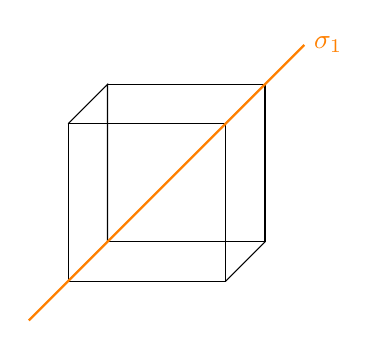
\begin{tikzpicture}[baseline=(current bounding box.south)]
                    % Coordinates of the vertices
                    \coordinate (A) at (0, 0);
                    \coordinate (B) at (0, 2);
                    \coordinate (C) at (2, 2);
                    \coordinate (D) at (2, 0);
                    \coordinate (E) at (0.5, 0.5);
                    \coordinate (F) at (0.5, 2.5);
                    \coordinate (G) at (2.5, 2.5);
                    \coordinate (H) at (2.5, 0.5);

                    % The cube
                    \draw (A) -- (B) -- (C) -- (D) -- cycle;
                    \draw (A) -- (E) -- (F) -- (B);
                    \draw (D) -- (H) -- (G) -- (C);
                    \draw (E) -- (F) -- (G) -- (H) -- cycle;

                    % The plane
                    \draw[thick,orange] (-0.5, -0.5) -- (3, 3);
                    \node[orange,right] at (3, 3) {$\sigma_1$};
                \end{tikzpicture}
                \hfil%
                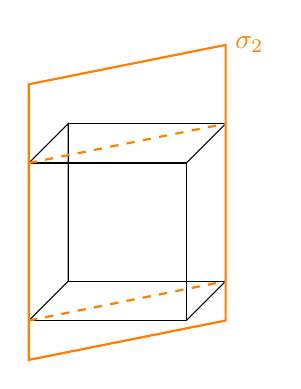
\begin{tikzpicture}[baseline=(current bounding box.south)]
                    % Coordinates of the vertices
                    \coordinate (A) at (0, 0);
                    \coordinate (B) at (0, 2);
                    \coordinate (C) at (2, 2);
                    \coordinate (D) at (2, 0);
                    \coordinate (E) at (0.5, 0.5);
                    \coordinate (F) at (0.5, 2.5);
                    \coordinate (G) at (2.5, 2.5);
                    \coordinate (H) at (2.5, 0.5);

                    % The cube
                    \draw (A) -- (B) -- (C) -- (D) -- cycle;
                    \draw (A) -- (E) -- (F) -- (B);
                    \draw (D) -- (H) -- (G) -- (C);
                    \draw (E) -- (F) -- (G) -- (H) -- cycle;

                    % The plane
                    \draw[thick,orange] (0, -0.5) -- (0, 3) -- (2.5, 3.5) -- (2.5, 0) -- cycle;
                    \draw[thick,dashed,orange] (A) -- (H);
                    \draw[thick,dashed,orange] (B) -- (G);
                    \node[orange,right] at (2.5, 3.5) {$\sigma_2$};
                \end{tikzpicture}
                \hfil
                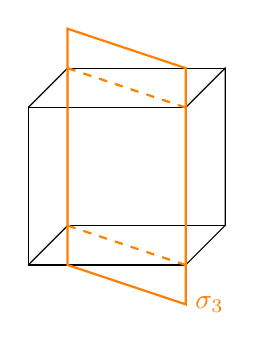
\begin{tikzpicture}[baseline=(current bounding box.south)]
                    % Coordinates of the vertices
                    \coordinate (A) at (0, 0);
                    \coordinate (B) at (0, 2);
                    \coordinate (C) at (2, 2);
                    \coordinate (D) at (2, 0);
                    \coordinate (E) at (0.5, 0.5);
                    \coordinate (F) at (0.5, 2.5);
                    \coordinate (G) at (2.5, 2.5);
                    \coordinate (H) at (2.5, 0.5);

                    % The cube
                    \draw (A) -- (B) -- (C) -- (D) -- cycle;
                    \draw (A) -- (E) -- (F) -- (B);
                    \draw (D) -- (H) -- (G) -- (C);
                    \draw (E) -- (F) -- (G) -- (H) -- cycle;

                    % The plane
                    \draw[thick,orange] (0.5, 3) -- (2, 2.5) -- (2, -0.5) -- (0.5, 0) -- cycle;
                    \draw[thick,dashed,orange] (C) -- (F);
                    \draw[thick,dashed,orange] (D) -- (E);
                    \node[orange,right] at (2, -0.5) {$\sigma_3$};
                \end{tikzpicture}
            \end{center}

            % TODO: graphs of $\sigma_1$, $\sigma_2$, and $\sigma_3$. 
    \end{remark}

    \begin{center}
        \begin{tikzpicture}
            % The cube expanded to 2D
            \draw (0, 0) -- (0, 2) -- (2, 2) -- (2, 0) -- cycle;
            \draw (0, 0) -- (-2, 0) -- (-2, 2) -- (0, 2);
            \draw (2, 2) -- (4, 2) -- (4, 0) -- (2, 0);
            \draw (4, 2) -- (6, 2) -- (6, 0) -- (4, 0);
            \draw (0, 2) -- (0, 4) -- (2, 4) -- (2, 2);
            \draw (2, 0) -- (2, -2) -- (0, -2) -- (0, 0);

            % Crosses on the cube
            \draw[dashed] (-2, 2) -- (0, 0) -- (2, 2) -- (4, 0) -- (6, 2);
            \draw[dashed] (-2, 0) -- (0, 2) -- (2, 0) -- (4, 2) -- (6, 0);
            \draw[dashed] (0, 4) -- (2, 2);
            \draw[dashed] (0, 2) -- (2, 4);
            \draw[dashed] (0, -2) -- (2, 0);
            \draw[dashed] (0, 0) -- (2, -2);

            % The vertices
            \node[graph-node,blue]   at (-2, 0) {};
            \node[graph-node,orange] at (-2, 2) {};
            \node[graph-node,orange] at (0, 0) {};
            \node[graph-node,blue]   at (0, 2) {};
            \node[graph-node,orange] at (2, 2) {};
            \node[graph-node,blue]   at (2, 0) {};
            \node[graph-node,orange] at (0, 2) {};
            \node[graph-node,blue]   at (2, 2) {};
            \node[graph-node,orange] at (2, -2) {};
            \node[graph-node,blue]   at (0, -2) {};
            \node[graph-node,blue]   at (4, 2) {};
            \node[graph-node,orange] at (4, 0) {};
            \node[graph-node,orange] at (6, 2) {};
            \node[graph-node,blue]   at (6, 0) {};

            % The centers of the crosses
            \node[graph-node,red] at (-1, 1) {};
            \node[graph-node,red] at (1, 1) {};
            \node[graph-node,red] at (1, 1) {};
            \node[graph-node,red] at (1, 3) {};
            \node[graph-node,red] at (1, -1) {};
            \node[graph-node,red] at (3, 1) {};
            \node[graph-node,red] at (5, 1) {};

            % The label $C$
            \node[magenta] at (1.5, 1) {$C$};
            \node[magenta] at (2.5, 1) {$\sigma_1C$};
            \node[magenta] at (1, 1.5) {$\sigma_2C$};
            \node[magenta] at (1, 0.5) {$\sigma_3C$};
            \node[magenta] at (0.5, 1) {$D$};
        \end{tikzpicture}
    \end{center}

    $D$ can be obtained by either $\sigma_3 \sigma_2 C$ or $\sigma_2 \sigma_3 C$. \[ \begin{matrix}
        \mathbb{R}^3 & \to & \mathbb{R}^3 & \to & \mathbb{R}^3 \\
        & \sigma_3 & & \sigma_2 & \\
        & \sigma_2 & & \sigma_3 &
    \end{matrix} \]

    Matrices are not commute, and thus these transformations may be different. We ask the questions: since $\sigma_2 \sigma_1$ and $\sigma_1 \sigma_2$ move the triangle $C$ in the same way, are they the same map?

    \begin{proposition}
        If $S, T: \mathbb{R}^3 \to \mathbb{R}^3$ preserve the coloured ube and send the triangle to the same place, then $S = T$ (as maps). 
    \end{proposition}

    \begin{proof}
        WTS $S = T$.

        \begin{remark}
            It is important that the triangle $C$ is a field of vectors. 
        \end{remark}
        Consider $o = (0, 0, \frac{1}{2})$, $b = (\frac{1}{2}, \frac{1}{2}, \frac{1}{2})$, and $y = (-\frac{1}{2}, \frac{-1}{2}, \frac{1}{2})$. 

        $Sb = Tb, So = To, Sy = Ty \implies (S - T)b = 0, (S - T)o = 0, (S - T)y = 0$.

        This implies $b$, $o$, and $y$ are in the kernel of $S - T$. 

        Moreover, $b, o, y$ are linearly independent since $\det \begin{bmatrix}
            \frac{1}{2} & 0 & -\frac{1}{2} \\
            \frac{1}{2} & 0 & -\frac{1}{2} \\
            \frac{1}{2} & \frac{1}{2} & \frac{1}{2}
        \end{bmatrix} \neq 0$.

        Thus, $\dim \ker (S - T) = 3$. Since $\dim \mathbb{R}^3 = 3$, $\ker (S - T) = \mathbb{R}^3$. Thus, $S - T = 0$.
    \end{proof}

    We can reach all 24 locations of the triangle $C$ by applying $\sigma_1$, $\sigma_2$, and $\sigma_3$ to the triangle $C$. Thus, there are 24 isometries that preserve the coloured cube. Moreover, we know that $3$ of them generates the set. It suffices to study these three isometries to understand the whole group.
\end{example}
\chapter{Introduction to Group}

\section{Introduction}

\begin{remark}
    What have we done so far: we have studied some \bred{objects} with some properties, and we have asked how can we operate in this object and preserve its property. 
\end{remark}

\begin{definition}[Group]\index{Group}\label{def:group}
    A \term{group} is a pair $(G, \cdot)$ where $G$ is a set and $\cdot$ is a binary operation on $G$ such that \[
        \begin{matrix}[cccc]
            \cdot & G \times G & \to     & G         \\
                  & (a, b)     & \mapsto & a \cdot b
        \end{matrix}
    \] such that \begin{listu}
        \item \textbf{Identity:} There exists an element $e \in G$ such that \[ e \cdot g = g \cdot e = a \quad \forall a \in G. \]
        \item \textbf{Inverse:} For every $g \in G$ there exists an element $h \in G$ such that \[ g \cdot h = h \cdot g = e. \]
        \item \textbf{Associativity:} For every $g, h, k \in G$ we have \[ g \cdot (h \cdot k) = (g \cdot h) \cdot k. \]
    \end{listu}
\end{definition}

\begin{definition}[Abelian Group]\index{Abelian Group}\label{def:abelian_group}
    A group $(G, \cdot)$ is called \term{abelian} if \[ g \cdot h = h \cdot g \quad \forall g, h \in G. \]

    This group is also called a \term{commutative group}.
\end{definition}

The term \textit{abelian} comes from the name of the Norwegian mathematician \href{https://en.wikipedia.org/wiki/Niels_Henrik_Abel}{Niels Henrik Abel}. He was the first to prove the impossibility of solving the general quintic equation in radicals. He also made important contributions to the study of elliptic functions, discovered Abelian functions, and many other important fields in mathematics.

\begin{example}
    We will consider the following ``toy"

    \begin{center}
        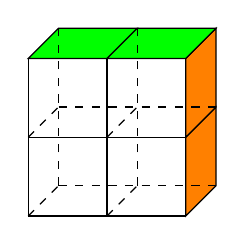
\begin{tikzpicture}
            \draw (0,0,0) -- (1,0,0) -- (1,1,0) -- (0,1,0) -- cycle;
            \draw (1,0,0) -- (2,0,0) -- (2,1,0) -- (1,1,0) -- cycle;
            \draw (0,1,0) -- (1,1,0) -- (1,2,0) -- (0,2,0) -- cycle;
            \draw (1,1,0) -- (2,1,0) -- (2,2,0) -- (1,2,0) -- cycle;

            \draw[fill=orange] (2,0,0) -- (2,0,-1) -- (2,1,-1) -- (2,1,0) -- cycle;
            \draw[fill=orange] (2,1,0) -- (2,1,-1) -- (2,2,-1) -- (2,2,0) -- cycle;

            \draw[fill=green] (0,2,0) -- (1,2,0) -- (1,2,-1) -- (0,2,-1) -- cycle;
            \draw[fill=green] (1,2,0) -- (2,2,0) -- (2,2,-1) -- (1,2,-1) -- cycle;

            % Dashed invisible lines
            \draw[dashed] (0,0,0) -- (0,0,-1);
            \draw[dashed] (1,0,0) -- (1,0,-1);
            \draw[dashed] (0,1,0) -- (0,1,-1);
            \draw[dashed] (1,1,0) -- (1,1,-1);
            \draw[dashed] (0,0,-1) -- (0,2,-1);
            \draw[dashed] (1,0,-1) -- (1,2,-1);
            \draw[dashed] (0,0,-1) -- (2,0,-1);
            \draw[dashed] (0,1,-1) -- (2,1,-1);
        \end{tikzpicture}

        The left side is red, the bottom is blue, and the back is yellow. 
    \end{center}

    We have $7$ operations \[
        V_1, V_2, H_1, H_2, V, H, R
    \] where \begin{listu}
        % TODO: add picture
        \item $V_1$ is the vertical flip of the first column
        \item $V_2$ is the vertical flip of the second column
        \item $H_1$ is the horizontal flip of the first row
        \item $H_2$ is the horizontal flip of the second row
        \item $V$ is the vertical flip of the whole cube
        \item $H$ is the horizontal flip of the whole cube
        \item $R$ is the rotation of the cube by $90^\circ$ around the vertical axis
    \end{listu}
    
    They satisfy \[
        {V_1}^2 = 1, {V_2}^2 = 1, {H_1}^2 = 1, {H_2}^2 = 1, V^2 = 1, H^2 = 1, R^4 = 1, 
    \]

    However, we have redundancies: \begin{listu}
        \item $V_1 V_2 = V_2 V_1 = V$
        \item $H_1 H_2 = H_2 H_1 = H$
        \item $V_1 H_1 = H_1 V_1 = R$
        \item $H_2 H_1 V_2 V_1 = R^2$
        \item $R^3 V_1 R = R^{-1} V_1 R = H_1$ 
        \item \dots
    \end{listu}

    We can flatten the cube into
    \begin{center} \begin{tabular}{c|c} 1 & 2 \\ \hline 3 & 4 \end{tabular} \end{center}

    Then, \begin{listu}
        \item $V_1 = (1, 4)$ 
        \begin{center} 
            \begin{tabular}{c|c} 1 & 2 \\ \hline 4 & 3 \end{tabular}
            \quad$\xrightarrow{V_1}$\quad
            \begin{tabular}{c|c} 4 & 2 \\ \hline 1 & 3 \end{tabular} 
        \end{center}

        \item $V_2 = (2, 3)$
        \begin{center} 
            \begin{tabular}{c|c} 1 & 2 \\ \hline 4 & 3 \end{tabular}
            \quad$\xrightarrow{V_2}$\quad
            \begin{tabular}{c|c} 1 & 3 \\ \hline 4 & 2 \end{tabular}
        \end{center}

        \item $H_1 = (1, 2)$
        \begin{center} 
            \begin{tabular}{c|c} 1 & 2 \\ \hline 4 & 3 \end{tabular}
            \quad$\xrightarrow{H_1}$\quad
            \begin{tabular}{c|c} 4 & 3 \\ \hline 1 & 2 \end{tabular}
        \end{center}

        \item $H_2 = (3, 4)$
        \begin{center} 
            \begin{tabular}{c|c} 1 & 2 \\ \hline 4 & 3 \end{tabular}
            \quad$\xrightarrow{H_2}$\quad
            \begin{tabular}{c|c} 1 & 2 \\ \hline 3 & 4 \end{tabular}
        \end{center}

        % \item $V = (1, 4)(2, 3)$

        \item $R = (1, 2, 3, 4)$
        \begin{center} 
            \begin{tabular}{c|c} 1 & 2 \\ \hline 4 & 3 \end{tabular}
            \quad$\xrightarrow{R}$\quad
            \begin{tabular}{c|c} 4 & 1 \\ \hline 3 & 2 \end{tabular}
        \end{center}
    \end{listu}

    We can verify that \[
        (1, 2, 3, 4) = (3, 4)(1, 4)(1, 2),
    \] which proposes that \[
        R = H_2 \circ V_1 \circ H_1
    \]

    % TODO: add picture
\end{example}

We have a group that is the one generator by the operations of the `toy` above. We have two models to understand the group: \begin{listo}
    \item The complete toy 
    \item The location code
\end{listo} What we have seen is that these two models are codify information in different ways. We can generate a map of the potential positions. 

% TODO: image

\begin{center}
    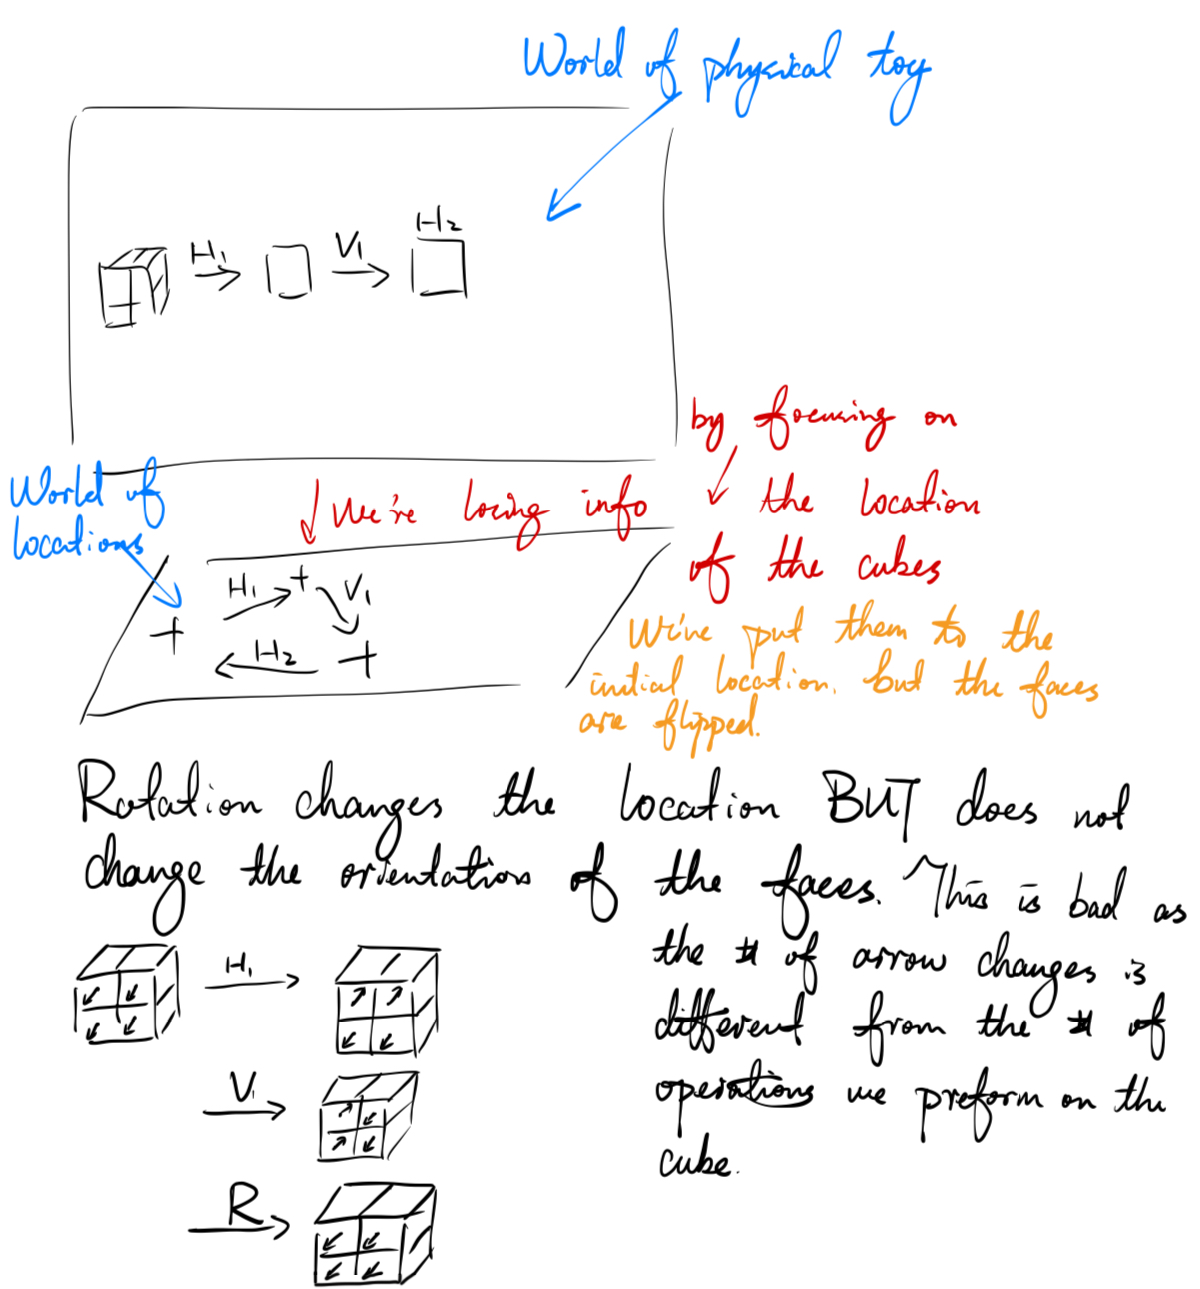
\includegraphics[width=0.55\linewidth]{figures/rubics-cube-1.png}
\end{center}

If we only allow $H_1, V_1, H_2, V_2$, then the locations are believable. The group they generate is $S_4$. 

\begin{remark}
    Think of $S_4$ independently. 

    We consider the permutations independently as a group. 

    \begin{center}
        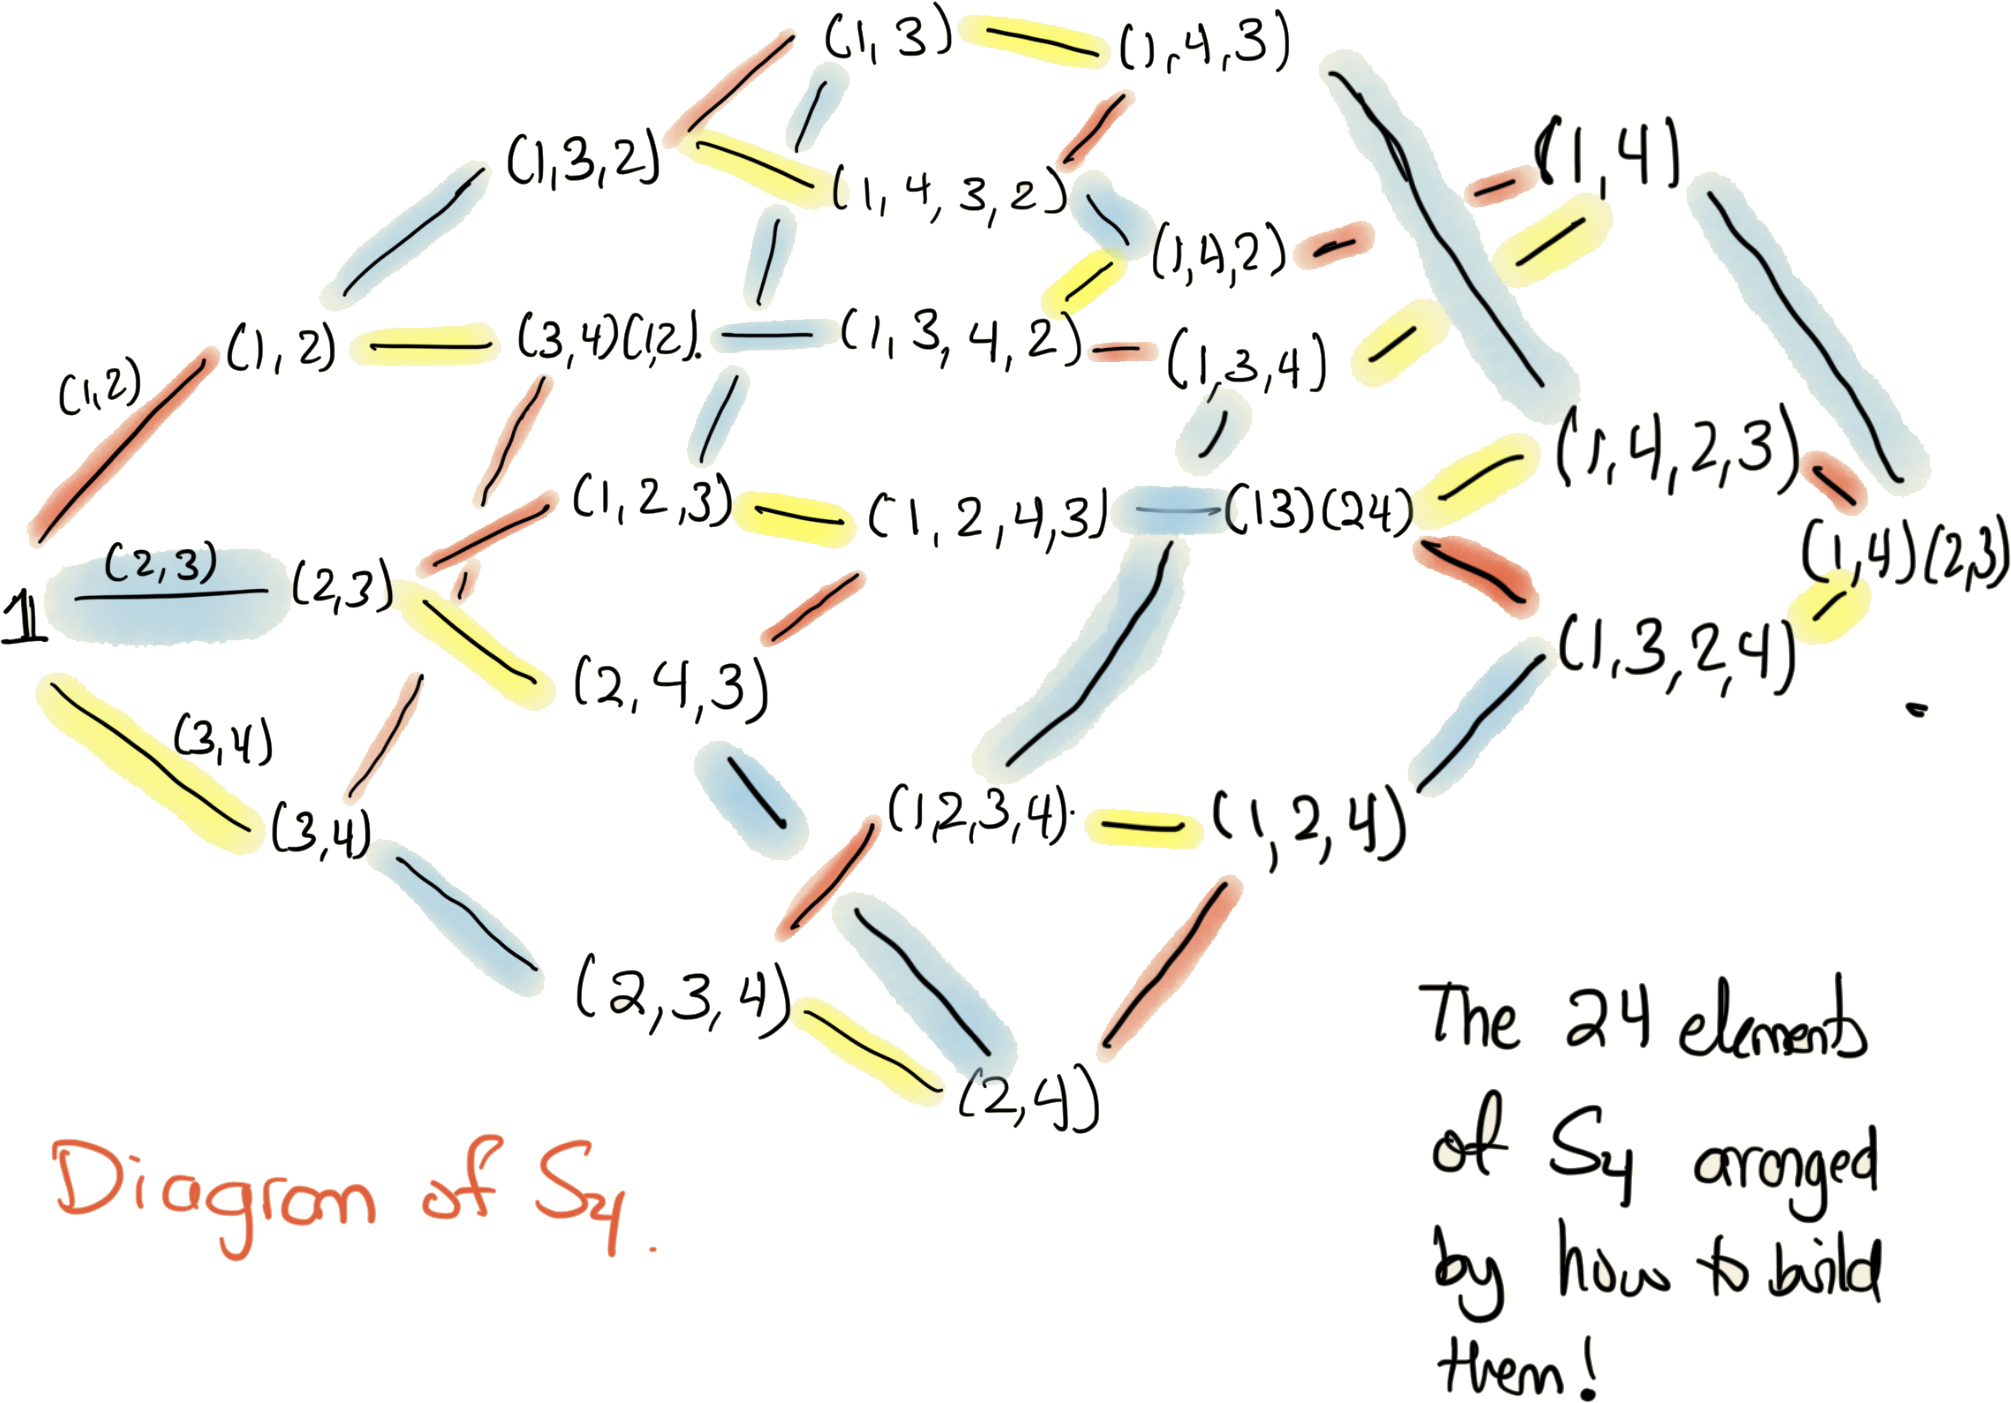
\includegraphics[width=0.55\linewidth]{figures/permutations-of-s4.png}
    \end{center}
\end{remark}

We want to merge $R$ with the rest of the operations. 

Consider \[
    H_1 R = R V_1 \qquad H_2 R = R V_2
\]

\begin{center}
    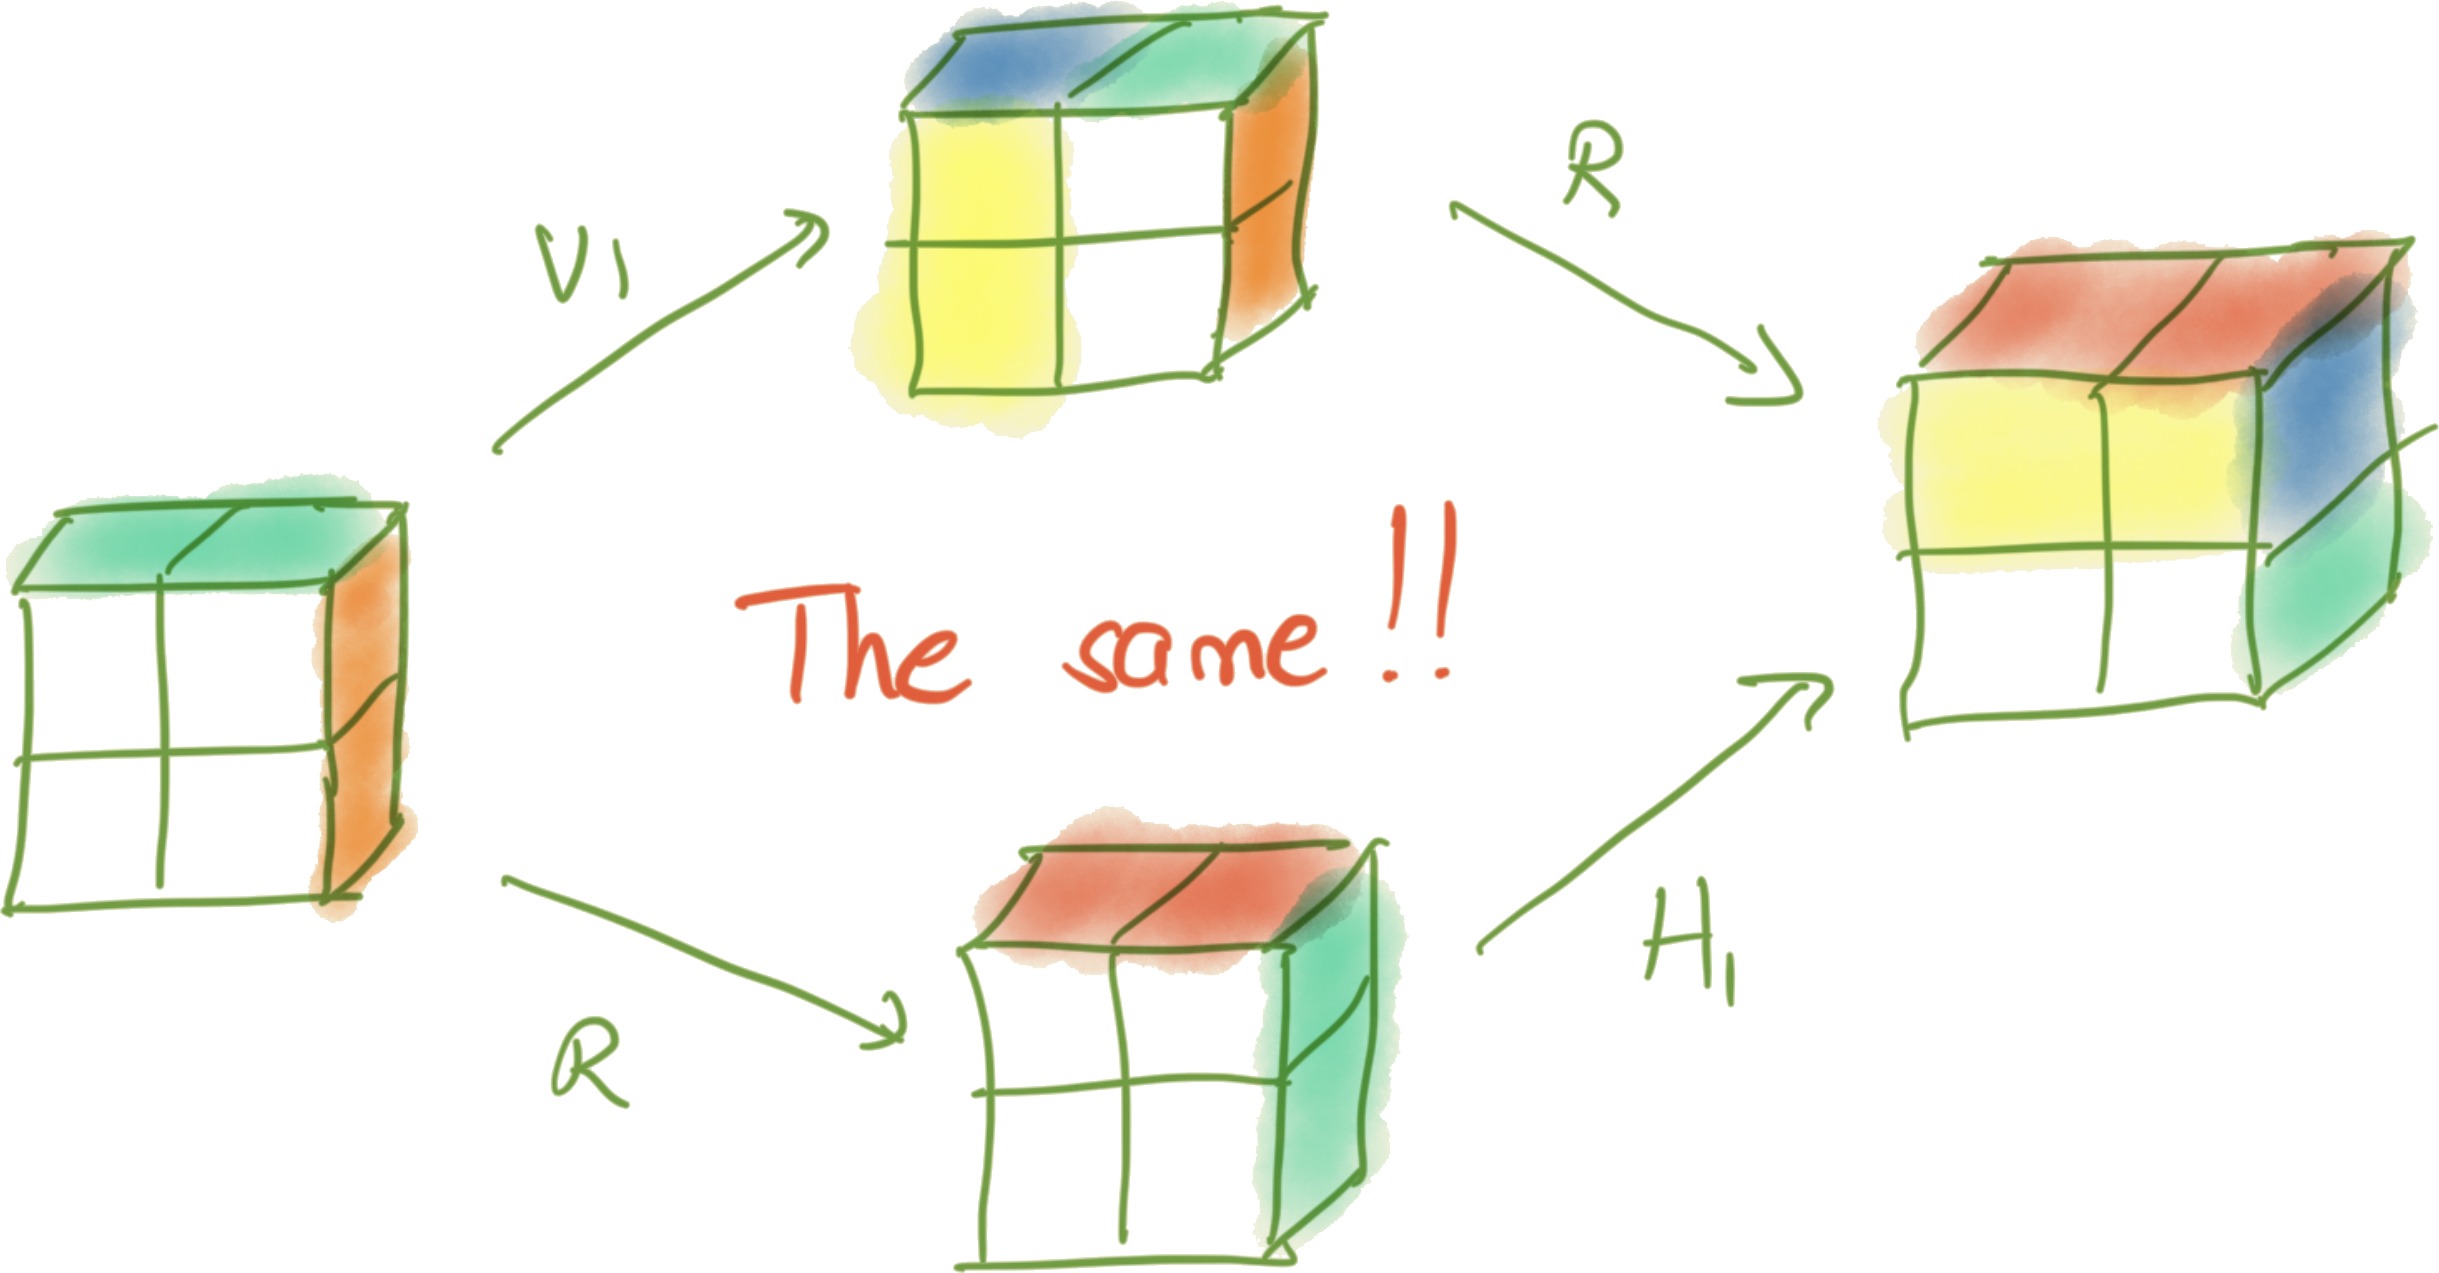
\includegraphics[width=0.45\linewidth]{figures/r-v1.png}
\end{center}

\begin{example}
    ``Simplify'' the instructions  \[
        R V_1 H_2 R V_2 H_1 H_2 R V_1 H_2
    \]

    Using the two equations above, 
    \begin{align*}
        R V_1 H_2 R V_2 H_1 H_2 R V_1 H_2
         & = R V_1 H_2 R V_2 H_1 {\color{red}R V_2} V_1 H_2             \\
         & = R V_1 H_2 R V_2 {\color{red}R V_1} V_2 V_1 H_2             \\
         & = R V_1 H_2 R {\color{red}R H_2} V_1 V_2 V_1 H_2             \\
         & = R V_1 H_2 {\color{red}V_1 V_2 H_1 H_2} H_2 V_1 V_2 V_1 H_2
         & (RR = V_1 V_2 H_1 H_2)                                       \\
    \end{align*}

    This way, we have moved all the ``noice'', $R$, to the last steps. 
\end{example}

\textbf{Fact:} All elements of the group can be written as \[
    X \sigma
\] where $X = 1 \text{ or } R$ and $\sigma \in S_4$. 

\begin{proposition}
    This writing is \bred{unique}. 
\end{proposition}

\begin{proof}
    Suppose $X_1 \sigma_1 = X_2 \sigma_2$. 

    \begin{listu}
        \item If $X_1 = X_2 = 1$, then $\sigma_1 = \sigma_2$.

        \item If $X_1 = X_2 = R$, then $R \sigma_1 = R \sigma_2$.

        Multiplying by $R^{-1}$, we have \[ \begin{aligned}[t]
            R^{-1} R \sigma_1 & = R^{-1} R \sigma_2 \\
            \sigma_1          & = \sigma_2
        \end{aligned} \]

        \item $X_1 = 1, X_2 = R$. Then, \[ \begin{aligned}[t]
            \sigma_1 & = R \sigma_2 \\
            \sigma_1 {\sigma_2}^{-1} & = R \sigma_2 {\sigma_2}^{-1} \\
            \sigma_1 {\sigma_2}^{-1} & = R
        \end{aligned} \] which means $R \in S_4$, which is impossible.
    \end{listu}
\end{proof}

These decomposition also has coordinates. $X$ uses the $R$-coordinate and $\sigma$ uses the $S_4$-coordinate.

We can write this as \[
    (1, \sigma) \in \pm 1 \times S_4
\]

However, note that $(s_1, \sigma_1) (s_2, \sigma_2) = (s_1 s_2, \sigma_1 \sigma_2)$ is \bred{not true}. The reason is because there is ``noice'' (procued by $R$) in the first coordinate.

\begin{center}
    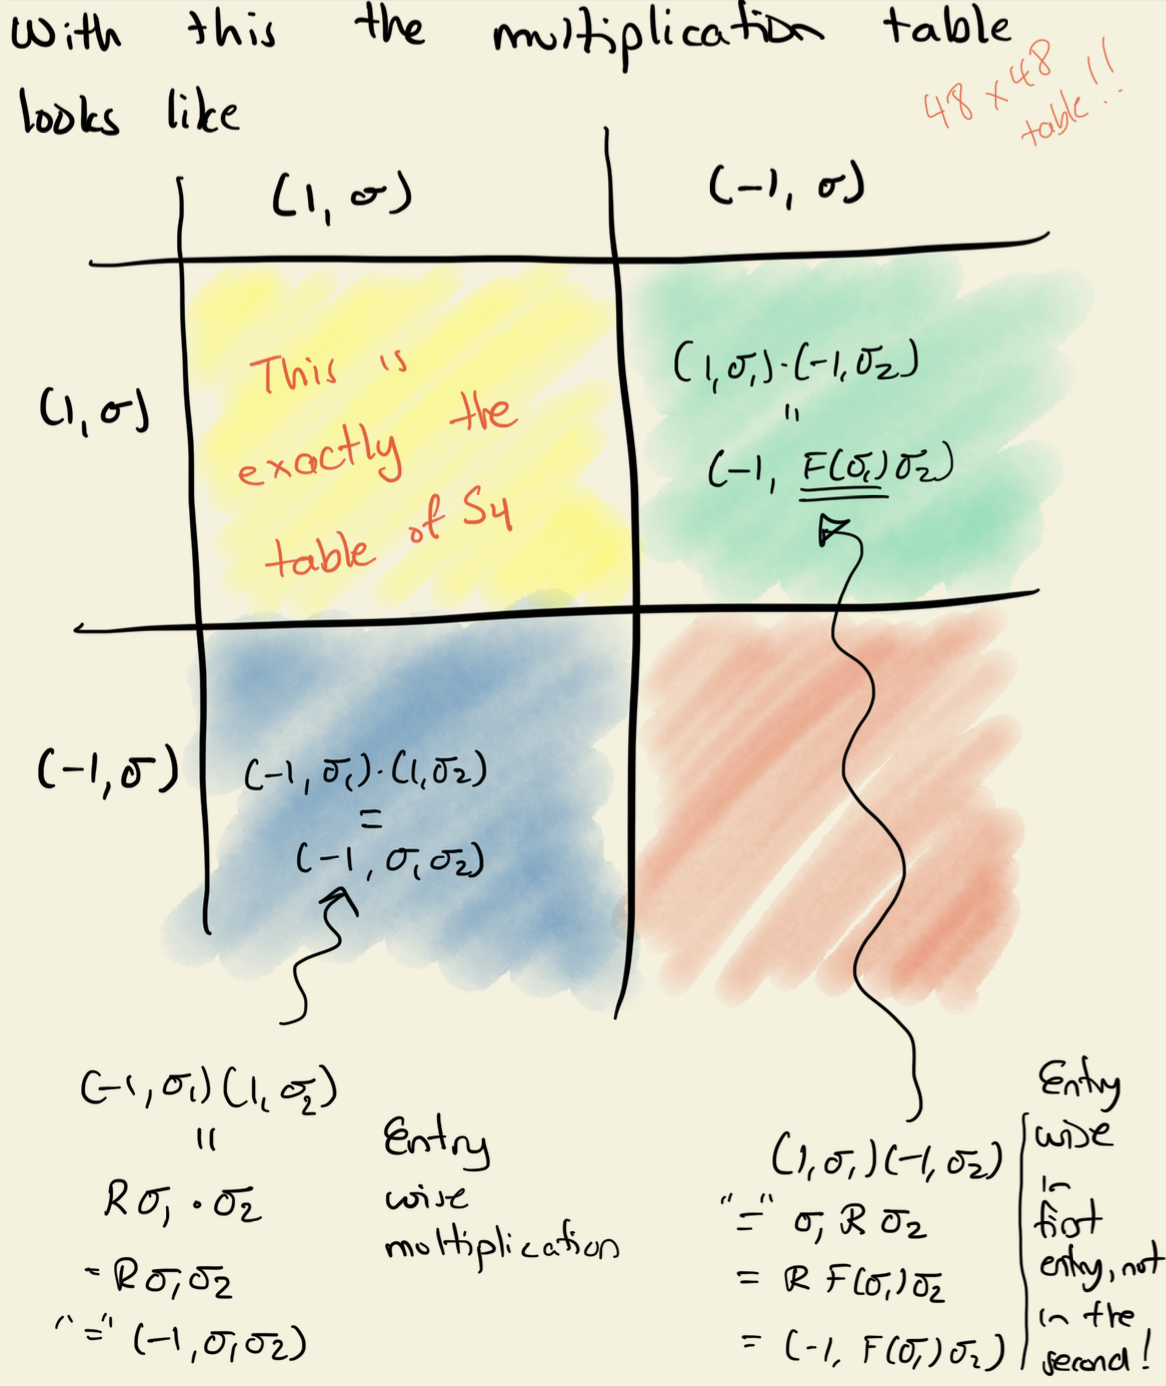
\includegraphics[width=0.67\linewidth]{figures/rotation_s4_table.png}
\end{center}

\part{Appendices}

\chapter*{Bibliography}
\addcontentsline{toc}{part}{Bibliography}
\nocite{*}
\printbibliography[heading=bibempty]

\cleardoublepage
\phantomsection
\setlength{\columnsep}{0.75cm}
\addcontentsline{toc}{part}{Index}
\printindex

\end{document}